\documentclass[licencjacka]{pracamgr}

\usepackage{polski}
\usepackage[utf8]{inputenc}
\usepackage{graphicx}

% Dane magistranta:

\author{Autorzy}

\nralbumu{Albumy}

\title{Framework oparty o wzorzec mikrousług na przykładzie portalu dla ZUS}

\tytulang{Project}

\kierunek{Informatyka}

% informatyka - nie okreslamy zakresu (opcja zakomentowana)
% \zakres{Tu wpisac, jesli trzeba, jedna z opcji podanych wyzej}

% Praca wykonana pod kierunkiem:
% (podać tytuł/stopień imię i nazwisko opiekuna
% Instytut
% ew. Wydział ew. Uczelnia (jeżeli nie MIM UW))
\opiekun{mgra Michała Możdżonka\\
  }

% miesiąc i~rok:
\date{Maj 2017}

%Podać dziedzinę wg klasyfikacji Socrates-Erasmus:
\dziedzina{ 
%11.0 Matematyka, Informatyka:\\ 
%11.1 Matematyka\\ 
%11.2 Statystyka\\ 
11.3 Informatyka\\ 
%11.4 Sztuczna inteligencja\\ 
%11.5 Nauki aktuarialne\\
%11.9 Inne nauki matematyczne i informatyczne
}

%Klasyfikacja tematyczna wedlug AMS (matematyka) lub ACM (informatyka)
\klasyfikacja{D. Software\\
  D.127. Ubezpieczenia społeczne}

% Słowa kluczowe:
\keywords{mikrousługi, SOA, trudne sprawy}

\begin{document}
\maketitle

%tu idzie streszczenie na strone poczatkowa
\begin{abstract}
  Potem dopiszemy.
\end{abstract}

\tableofcontents
%\listoffigures
%\listoftables

%\chapter{Organizacja pracy}

%Pierwszym poważnym wyzwaniem, przed którym staneliśmy, była organizacja pracy zespołu. Każdy członek zespołu
%pochodzi z innego miasta i uczęszcza na inne zajęcia, ponadto część członków pracuje. Znalezienie pory i dnia
%tygodnia, w którym moglibyśmy się spotykać, stanowiło spore wyzwanie. W gospodarowaniu czasem i ustalaniu terminów
%spotkań z klientem bardzo nam pomogło doodle. % Mądrze rozwinąć!
%Komunikacja między członkami zespołu odbywała się głównie przez internet, przy pomocy facebooka %i slacka.
%Projekt prowadziliśmy w lekko zmodyfikowanej zwinnej metodyce opracowanej specjalnie na potrzeby naszego klienta.

\chapter*{Wprowadzenie}\label{r:wstep}
\addcontentsline{toc}{chapter}{Wprowadzenie}

Celem naszego projektu było stworzenie prototypu internetowego frameworka do komunikacji obywatela z urzędami
podobnego do Platformy Usług Elektronicznych ZUS \cite{zuspue}, a następnie zaimplementowanie na niej kilku wybranych przypadków użycia. Dzięki temu petent chcący
coś załatwić w urzędzie nie będzie musiał wychodzić z domu. Pewną inspiracją do stworzenia takiego systemu był
rządowy portal obywatel.gov.pl \cite{mcobywatel}.

Wyzwaniem, które należało uwzględnić w fazie projektowania, był szeroki zakres użytkowników systemu: od zwykłych
obywateli, poprzez urzędników, aż po przedsiębiorców. Każda z tych grup użytkowników miałaby zupełnie inne uprawnienia:
byłoby co najmniej niestosowne, gdyby przedsiębiorca wnioskowałby o urlop macierzyński dla prowadzonej przez siebie
firmy. Podobnie obywatel nie powinien mieć możliwości przyznania sobie emerytury lub renty (o ile nie jest urzędnikiem). Główne przypadki użycia systemu sprowadzałyby się do trzech wariantów: wypełniania wniosków, sprawdzania
odpowiedzi na wypełniony wniosek i rozpatrywania wniosków. Pobocznymi przypadkami byłyby: rezerwacja terminu wizyty w
urzędzie w przypadku nadzwyczaj zawiłych spraw, prezentacja różnych danych użytkownikowi (np. stanu ubezpieczenia,
wysokości przyznanej renty lub wymaganego ustawowo pouczenia) oraz wymiana korenspondencji z urzędnikiem. W obecnie
istniejącym systemie PUE jest jeszcze jeden przypadek użycia: czat z konsultantem. Nasza platforma powinna umożliwiać
stosunkowo prostą realizację niemal wszystkich spośród wymienionych wyżej przypadków użycia.

Kiedy użytkownik zaloguje się do naszego serwisu powinien zobaczyć pulpit, na którym wyświetlone są ,,kafelki''
odpowiadające poszczególnym usługom. Kliknięcie na wybrany kafelek powinno wyświetlić bardziej szczegółowy widok
odpowiadający podjętej akcji. Szczególnym życzeniem naszego klienta było, by architektura naszej aplikacji była
oparta na mikrousługach. Każda mikrousługa otrzymywałaby na wyłączność fragment pulpitu ograniczony do kafelka,
z możliwością przełączenia do trybu pełnoekranowego, gdzie przejmowałaby wtedy kontrolę nad większością wyświetlanego
obszaru. Aby to umożliwić, należało opracować ustandaryzowany i łatwo rozszerzalny interfejs do komunikacji między
cienkim klientem a mikrousługą. Preferowane było rozwiązanie, w którym komunikacja odbywałaby się bez pośrednictwa
serwera serwującego stronę internetową. Zamiast tego wykonywane byłyby asynchroniczne zapytania do mikrousługi (być
może poprzez warstwę integracji).

Postawione przed nami wymagania były głównie natury niefunkcjonalnej. Dołączanie kolejnej usługi do systemu
powinno być maksymalnie proste. Na tę prostotę składałby się ustandaryzowany interfejs do komunikacji pomiędzy
poszczególnymi usługami oraz modułowy i łatwo rozszerzalny interfejs użytkownika.
To pozwoli nam stosunkowo małym kosztem podłączać i odłączać kolejne usługi wraz z
rozwojem cyfrowej administracji. Usługi powinny tworzyć jeden ekosystem, z którego nie wychodziłby użytkownik. System
powinien być w dużej mierze odporny na awarie i zachowywać spójność oraz poprawność przechowywanych danych obywateli.
W szczególności powinny być spełnione normy ,,12 Factor App'' \cite{tfa}, w tym ta mówiąca, że awaria jednego serwera
lub usługi nie powinna wpływać na działanie pozostałych, niezależnych od niej udostępnianych usług.
Rozwój i utrzymanie platformy powinien być możliwy także dla słabiej wykształconych lub mniej doświadczonych
programistów, których nie pociągają uroki życia w dużym mieście. W ten sposób nasz projekt realizowałby plan
zrównoważonego rozwoju, zapobiegając zwijaniu się polski lokalnej, a z drugiej strony prowadziłby do wymiernych
oszczędności na wynagrodzeniach.

Innym istotnym aspektem naszego projektu było zerwanie z wizerunkiem ZUSu jako instytucji przestarzałej, niewydolnej
i pochodzącej ze słusznie minionego ustroju. Szata graficzna naszej platformy powinna być przyjemna dla oka, a układ
graficzny elementów logiczny, prosty do zrozumienia i konsekwentny. Użytkownik nie może być bombardowany zagadkowo
brzmiącymi komunikatami o ,,wchodzeniu na poziom bezpieczeństwa 1'' i ,,zamiarze korzystania z usług biznesowych''.
W żadnym przypadku praca z naszym systemem nie
powinna przypominać interakcji ze znudzonym i ślamazarnie wykonującym swoje obowiązki urzędnikiem, a to nakłada na
nas obowiązek rozwiązania problemu skalowalności aplikacji.

W związku z tym, że projektowaliśmy system dla administracji państwowej z którego będą korzystać miliony obywateli,
musieliśmy bardzo ostrożnie dobierać technologie, z których korzystaliśmy. Wybranie rozwiązania opartego na
niekorzystnej licencji mogło się w przyszłości srogo zemścić w postaci konieczności zapłacenia ogromnej opłaty
licencyjnej, wyłączenia usługi i przebudowania jej na nowo, udostępnienia części systemu na licencji open source, a
nawet konieczności nieodpłatnego przekazania przechowywanych danych obywateli licencjodawcy. Preferowane były
rozwiązania które albo były darmowe, albo do których nasz klient posiadał licencje (m. in. IBM DB2, komercyjna wersja PostgreSQL oraz cała gama produktów firmy Microsoft). W miarę możliwości
powinniśmy korzystać z nowoczesnych, przyszłościowych i rozwijanych technologii, tak, by odsunąć jak najdalej w
przyszłość konieczność przebudowy systemu z powodu zmieniających się trendów i narastającego długu technologicznego.

%Elementy, które powinny się znaleźć w dokumencie opisującym wizję to:
%Opis rozwiązania, Korzyści biznesowe, Wizja projektu i zakres, Analiza korzyści, Wymagania biznesowe, Wymagania użytkowników, Wymagania operacyjne, Wymagania systemowe, Wymagania bezpieczeństwa, Zakres projektu, Cele biznesowe, Cele techniczne, Kryteria operacyjne, Ograniczenia, Definicja profili użytkowników, Analizy użytkowania, Scenariusze wykorzystania

\chapter{Architektura aplikacji}

Zdecydowaliśmy się przenieść środek ciężkości naszego projektu w stronę warstwy integracji klienta z backendem. Ustalono, że do osiągnięcia sukcesu wystarczy spełnienie następujących warunków: %TODO
\begin{itemize}
	\item Zrobicie warstwę FE + BFF w ten sposób, że zostanie zrobione środowisko Web Style Guide z podstawowymi i złożonymi kontrolkami oraz z generacją kodu.
	\item Następnie użytkownik będzie mógł sam wyklikać kontrolki i ustawić to w dashboardy.
	\item Na końcu chciałbym mięc zrobiony mockup pue.zus.pl wyklikany w ten sposób.
\end{itemize}

\section{Interfejs użytkownika}
TODO

Tego chcemy uniknąć:\\
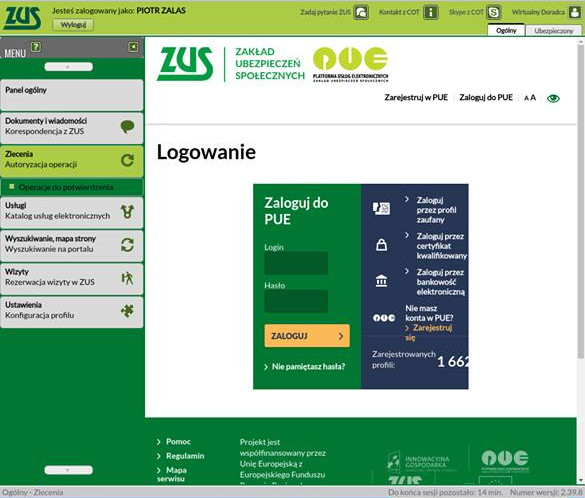
\includegraphics[width=\textwidth]{obrazki/logowaniezle.jpg}

\section{Integrator}
Integrator - autodiscovery usług, możliwość spinania różnych interfejsów gRPC, WSDL. 
Z uwagi na to, że dane przechodzą przez niego w postaci nieszyfrowanej można
go podłączyć do IDSa wykrywającego anomalie w przesyłanych danych i w ten sposób
zapobiegać masowemu wyciekowi wrażliwych danych lub atakom hakerskim. Stanowi też
dodatkową linię obrony, którą musi sforsować potencjalny haker. Dzięki temu system jest
odporniejszy na błędy popełnione w serwerach mikrousług, a w przypadku wykrycia
jakiejś luki można ad-hoc wprowadzić łatkę bezpieczeństwa w serwerze pośredniczącym
zamiast łatać wszystkie podatne serwery mikrousług.

W naszej architekturze mikrousług potrzebowaliśmy jakiejś metody komunikacji pomiędzy poszczególnymi mikrousługami.
Na początku nasza uwaga została przykuta przez szyny danych jako standardowe rozwiązanie korporacyjne wykorzystywane
przy integracji usług. Nasz klient jest w posiadaniu licencji na szynę danych WebMethods i to ją jako pierwszą
rozpatrywaliśmy. Niestety, dostępna publicznie internetowa dokumentacja tego rozwiązania ograniczała się do kilku
broszurek reklamowych i luźnych sloganów. Z czystej ostrożności zrezygnowaliśmy z tego oprogramowania, gdyż nie
mieliśmy absolutnie żadnej gwarancji, że wyczytane hasła reklamowe mają jakiekolwiek pokrycie w rzeczywistości.
Do kolejnej grupy sprawdzonych szyn danych należały rozwiązania takie jak: WSO2, Talend, Mule. Możliwości, które
oferowały wyglądały na obiecujące, ale zupełnie niepasujące do specyfiki naszego projektu. Jednym z celów naszej
platformy było opracowanie interfejsu, który pozwalałby na możliwie łatwe, automatyczne wpinanie i wypinanie
mikrousług. Nijak do tak postawionego celu miała się konieczność konfigurowania szyny danych przez panel wystawiony w sieci
WWW lub wręcz przy pomocy specjalnego środowiska programistycznego takiego jak Eclipse, z obowiązkową fazą kompilacji
i wgrywania na serwer. 

Rozwiązaniem wartym wspomnienia jest Zato, dość osobliwa szyna danych rozwijana przez osobę o polsko brzmiącym nazwisku. Jej głównymi cechami są skalowalność, możliwość rekonfiguracji w locie oraz bardzo dobra integracja z językiem python, co miało dla nas niebagatelne znaczenie na etapie wczesnych analiz. W zasadzie cała logika realizowana przez tę szynę danych mogła być zapisana w postaci skryptu pythona, co otwierało nas na zupełnie nowe możliwości integracji mikrousług. Rozważaliśmy scenariusz, w którym szyna danych odpowiadałaby za wykrywanie działających mikrousług, trzymanie ich spisu i metadanych z nimi powiązanych oraz rozgłaszanie tegoż spisu do warstwy prezentacji i innych mikrousług. Zrezygnowaliśmy z tego podejścia jako naruszającego zasadę separacji odpowiedzialności oraz wskutek zmian projektowych - rezygnacji z frameworka django, pyramid i podobnych na rzecz Angulara. Jak się potem okazało, istnieje już rozwiązanie które realizuje wyżej wymienione scenariusze - Apache Zookeeper.

Niepowodzenia przy poszukiwaniu odpowiadającej nam szyny danych skierowały nas w kierunku innych rozwiązań, takich jak
kolejki komunikatów. Głównym wymaganiem jakie postawiliśmy była bardzo duża odporność na różnego rodzaju błędy i
awarie. W idealnym modelu każda wiadomość w kolejce powinna mieć trzy stany: do przetworzenia, w trakcie przetwarzania, wykonany. Celem takiego modelu jest, by w przypadku awarii jednego serwera usługi jego zadanie było transparentnie przekazane serwerowi zastępczemu, bez przerywania operacji. Udało nam się znaleźć tylko jedną kolejkę spełniającą to wymaganie - Beanstalkd.

Innym sposobem osiągnięcia niezawodności może być kolejka ukryta wewnątrz mikrousługi, która w razie awarii jednego serwera pozwalałaby na odczytanie zadania przez inny serwer i dokończenie go. Niestety wtedy mogą mieć miejsce problemy z atomowością operacji. Przykładowo, w sytuacji gdy zadanie w kolejce zostało oznaczone jako wykonane, ale usługa wywołująca nie otrzymała jeszcze odpowiedzi nastąpi awaria wywoływanej mikrousługi, może dojść do duplikacji wykonanej operacji lub rozspójnienia danych.

Jeszcze innym, ciekawym podejściem byłoby zastosowanie usługi udostępniającej niezawodny dostęp do czegoś w rodzaju dziennika. Wtedy moglibyśmy stosunkowo małym kosztem zaimplementować mechanizmy stosujące transakcyjność rodem z relacyjnych baz danych. Przykładami takich usług są DistributedLog i Kafka. Poszczególne mikrousługi monitorowałyby dziennik i z niego pobierały zmiany, a następnie reagowały na nie poprzez podjęcie jakiejś akcji. Można sobie wyobrazić dwa sposoby wykorzystania takiego dziennika. Pierwszy polegałby na tym, że wszystkie dokonane zmiany są atomowo publikowane w jednej dużej paczce, która musiałaby być potem rozpakowywana, a poszczególne zmiany wyłuskiwane. Drugim sposobem byłoby stworzenie dużej ilości dzienników na każdy rodzaj zdarzenia, a każda operacja byłaby wykonywana w małych krokach, w sposób potokowy.

\section{Mikrousługi}
TODO

\chapter{Wykorzystane technologie}\label{r:tech}

\section{Języki programowania}
Python, Java, Node.js, typescript

\section{Angular 2}

Do tworzenia cześć wizualnej oraz logiki bezpośrednio z nią związanej, użyliśmy frameworka Angular2. Jest to narzędzie stworzone przez Google, opierające się
na Type Script - języku będącym nadzbiorem Java Script. W stosunku do js główną funkcjonalnością ts jest dodanie obiektowości, jednakże można stwierdzić,
że wszystko co związane z obiektowością w ts to tylko lukier syntaktyczny, ponieważ w ts koniec konców jest przetłumaczony do czystego js. Ts implementuje większość
funkcjonalności, które język obiektowy powinien oferować - możliwe jest dziedziczenie, tworzenie interfesjów, konstruktory itp. Ciekawą opcją są dekoratory, czyli
odzobniki klas. Dekoratory (szerzej opisane w dalszej części pracy) pozwalają na zmianą ``zachowania'' klasy już w trakcie kompilacji.

\section{Bootstrap}

Za wygląd strony odpowiada HTML5, połączony z Bootstrapem. Bootstrap to zbiór gotowych komponentów wizulanych, pozwalający, bez zbędnego wnikania
w stronę ``artystyczną'', tworzyć strony estetyczne oraz wygodne w użyciu. Jako, że tematem naszej pracy nie jest projektowanie stron internetowych,
użyliśmy gotowej skórki - sbAdmin2. Właściwie, lepszym określeniem, jest użycie sbAdmin2 jako punktu wyjścia, ponieważ liczba wprowadzliśmy
liczne zmiany w wyglądzie platformy.

\section{Express.js}

\section{ZooKeeper}

Jednym z elementów wizji naszego systemu był fakt, że poszczególne usługi
powinny możliwie prosto ,,wpinać się'' w system. Serwer mikrousługi w trakcie
uruchamiania dopisywałby do globalnej konfiguracji wpisy związane z prowadzoną
przez siebie działalnością, takie jak adresy pod którymi przyjmuje zapytania
albo pozycje w menu widocznym dla użytkownika, które prowadzą do poszczególnych
usług biznesowych. Doszliśmy do wniosku, że nasze oczekiwania można sprowadzić
do trzech wymagań:
\begin{itemize}
	\item przechowywania konfiguracji w drzewiastej strukturze
	\item automatycznego usuwania dokładnie określonych wpisów w przypadku
	utraty dowolnego serwera mikrousługi
	\item automatyczną replikację danych
\end{itemize}
Istnieją rozwiązania, które przynajmniej częściowo spełniają nasze wymagania i
teraz je przedstawimy.

Najbliższy naszym potrzebom był serwer Apache ZooKeeper \cite{zookeeper} w
połączeniu z biblioteką Apache Curator \cite{curator}. Dane na serwerze
ZooKeeper są trzymane w drzewiastej strukturze. Każdy węzeł może zawierać dowolny
ciąg bajtów ograniczony do rozmiaru ok. 1 Mb. Węzły są wersjonowane, a dostęp
do nich jest kontrolowany przez mechanizm ACL. Na każdym węźle można ustawić
obserwatora (ang. \textit{watch}), który w przypadku jakiejkolwiek modyfikacji
węzła powiadamia klienta o zmianie. Oprócz tego, każdy węzeł może mieć ustawione
dwie dodatkowe flagi. Pierwsza to \textit{ephemeral}, która oznacza, że węzeł ma
istnieć tylko do czasu zakończenia sesji klienta, który utworzył dany węzeł.
Ta własność jest szczególnie interesująca w kontekście automatycznego
wyrejestrowywania usługi która kończy swe działanie i nie ma możliwości
powiadomienia serwera o tym fakcie. Druga flaga to \textit{sequence}. Mówi ona,
że należy do nazwy tworzonego węzła dopisać rosnący numer. Ma to zastosowanie we
wszelkiego rodzaju kolejkach, algorytmach synchronizujących i przy wyborze
lidera \cite{curatorlock}.

\subsection{Curator}
Biblioteka Curator upraszcza wiele aspektów związanych
z wykorzystaniem ZooKeepera, między innymi rejestrację serwerów mikrousług,
zapewnia implementację najczęściej wykorzystywanych algorytmów synchronizujących
oraz łatwe buforowanie drzewa węzłów wraz z automatycznym pobieraniem zmian. W
trakcie prac nad integratorem okazało się, że oferowane możliwości znacznie przekraczają
nasze potrzeby.

\subsection{Kazoo}
Zk dla pythona

\section{Django}

\section{Play Framework}

\section{GRPC}

\section{SQLite}

W naszym projekcie rodzaj użytej bazy danych nie miał większego znaczenia, gdyż dostęp do niej odbywa się poprzez
wyspecjalizowaną usługę zapewniającą dostęp do danych lub w ramach jednej mikrousługi, gdzie służy jako tymczasowe
składowisko informacji potrzebnych przy wykonywaniu operacji. W takim modelu rodzaj użytej bazy danych jest
transparentny dla usługi wywołującej. Z uwagi na prototypowych charakterze naszego projektu poprzestaliśmy na
bazie SQLite, jako że znakomicie integruje się on z Django, ponadto zastąpienie go PostgreSQLem jest praktycznie bezkosztowe.

\chapter{Frontend}\label{r:fe}

\section{Tworzenie mockupów}
Tutaj opis wszystkich stworzonych podstron
\section{Stworznie systemu komponentów}
Opis posczególnych komponentów, oraz całej idei architektury tego rozwiązania.
\section{System tworzenia automatycznej dokumentacji}
Opis dekoratorów.
\section{Edytor}
TODO
\section{Platforma developera}
Sposób dodawania mikrosusług, style guide.

\chapter{Integrator i mikrousługi}\label{r:ims}

\chapter{Obserwator emerytalny}
Z uwagi na bardzo niepewny charakter naszego projektu i trudności związane z
formalnym rozliczeniem naszej pracy zdecydowaliśmy się wykonać niejako poza
głównym projektem serwis ,,Obserwator emerytalny''.

\chapter{Wkład poszczególnych członków zespołu w projekt}\label{r:wklad}
TODO
\appendix
\chapter{Spis zawartości dołączonej płyty CD}\label{r:spis}
Dokładny spis zawartości towarzyszącej płytki (p. dalej). To bardzo ważne, proszę zapisać jako osobny rozdział (czyli np. nie podrozdział). Płytka CD/DVD/Blu-ray/...

Zawiera:\\
Pełną dokumentacją projektu w łatwo dającym się odczytać formacie (najlepiej pdf + źródło).
Program (w postaci źródłowej i potencjalnie umożliwiającej uruchomienie, to może oznaczać np. dostarczenie stosownych plików makefile, pomocniczych plików z danymi, opisu instalacji itp.).
Wszelkie inne dokumenty powstałe podczas zajęć (np. teksty prezentacji, teksty pracy z poprzedniego dużego punktu, itp.).

Płyta jest częścią pracy - trzeba tyle płyt co drukowanych egzemplarzy pracy. Płytkę trzeba przymocować do pracy, tak by a) nie wypadała b) dało się ją wyjąć i odczytać w komputerze :).

\begin{thebibliography}{99}
\addcontentsline{toc}{chapter}{Bibliografia}

\bibitem[DOZ]{zusdoz} ZUS, \textit{Dokumentowanie okresów zatrudnienia oraz
	wynagrodzenia}, http://www.zus.pl/files/Dokumentowanie\_okres\%C3\%B3w\_zatrudnienia.pdf

\bibitem[TFA]{tfa} Autor nieznany, \textit{The Twelve-Factor App}, https://12factor.net/

\bibitem[SDM]{govsm} Autor nieznany, \textit{Government Service Design Manual},
https://www.gov.uk/service-manual/index.html

\bibitem[MSV]{microsvc} Chris Richardson, \textit{Microservice architecture patterns and best practices},
http://microservices.io/

\bibitem[MCO]{mcobywatel} Ministerstwo Cyfryzacji, \textit{Portal Rzeczypospolitej Polskiej - Opis projektu},
https://mc.gov.pl/projekty/portal-rzeczypospolitej-polskiej/opis-projektu

\bibitem[PUE]{zuspue} ZUS, \textit{Platforma Usług Elektronicznych},
http://pue.zus.pl/

\bibitem[RDL]{redislock} Redis, \textit{Distributed locks with Redis},
https://redis.io/topics/distlock

\bibitem[RDS]{redisson} \textit{Redisson},
http://redisson.org/

\bibitem[AZK]{zookeeper} Apache, \textit{Apache ZooKeeper},
https://zookeeper.apache.org/

\bibitem[ACU]{curator} Apache, \textit{Apache Curator},
http://curator.apache.org/

\bibitem[HTL]{redisbad} Martin Kleppmann, \textit{How to do distributed locking},
http://martin.kleppmann.com/2016/02/08/how-to-do-distributed-locking.html

\bibitem[CLK]{curatorlock} Apache, \textit{Apache Curator - Shared Lock},
http://curator.apache.org/curator-recipes/shared-lock.html

\bibitem[Fowler]{fowlermicroservices} Martin Fowler, \textit{Microservices},
https://martinfowler.com/articles/microservices.html

\end{thebibliography}

\end{document}
